% NetraRakshak — IEEE conference-format project report.
% Compiles with the official IEEEtran class when it is installed (e.g. on Overleaf or a full TeX Live);
% otherwise it falls back to a two-column article layout that follows IEEE conference conventions.
\IfFileExists{IEEEtran.cls}{%
  \documentclass[conference]{IEEEtran}
  \newcommand{\usingieeetran}{}
}{%
  \documentclass[10pt,twocolumn,letterpaper]{article}
  \usepackage[top=0.75in,bottom=1in,left=0.625in,right=0.625in,columnsep=0.25in]{geometry}
  \usepackage{mathptmx}
  \usepackage[small,bf]{caption}
  \usepackage{titlesec}
  \renewcommand{\thesection}{\Roman{section}}
  \renewcommand{\thesubsection}{\Alph{subsection}}
  \titleformat{\section}{\centering\normalfont\scshape}{\thesection.}{0.5em}{}
  \titleformat{\subsection}{\normalfont\itshape}{\thesubsection.}{0.5em}{}
  \titlespacing*{\section}{0pt}{10pt}{5pt}
  \titlespacing*{\subsection}{0pt}{7pt}{3pt}
  \newenvironment{IEEEkeywords}{\noindent\textbf{\textit{Index Terms}---}\bfseries\small}{\par\medskip}
  \renewenvironment{abstract}{\noindent\textbf{\textit{Abstract}---}\bfseries\small}{\par\medskip}
  \newcommand{\IEEEauthorblockN}[1]{##1\\}
  \newcommand{\IEEEauthorblockA}[1]{\small\itshape ##1}
}
\usepackage{graphicx}
\usepackage{booktabs}
\usepackage{amsmath,amssymb}
\usepackage{cite}
\usepackage{tikz}
\usetikzlibrary{positioning,arrows.meta,fit,backgrounds,calc}
\usepackage[hidelinks]{hyperref}
\usepackage{url}

\begin{document}

\title{NetraRakshak: A Clinician-Supervised, AI-Assisted Retinal Screening Platform for Diabetic Retinopathy}

\author{\IEEEauthorblockN{Oindreela Saha}
\IEEEauthorblockA{NetraRakshak Project\\ India}}

\date{}
\maketitle

\begin{abstract}
Diabetic retinopathy (DR) is a leading cause of preventable vision loss, and screening programmes in India are limited
by the availability of ophthalmologists rather than by imaging. This paper presents NetraRakshak, a multi-tenant
software platform that carries a colour fundus photograph from capture to a clinician-signed screening report. Each
image first passes an automatic quality gate of ten computer-vision checks; gradable images are then graded on the
five-level International Clinical DR scale by an EfficientNet-B0 network with temperature-scaled confidence, an
entropy-based uncertainty rule that returns ``inconclusive --- human review required'', and Grad-CAM explanations. An
ophthalmologist accepts, modifies or rejects every AI suggestion before a report can be approved. Trained on the
APTOS 2019 dataset (3,662 images), the model achieved, on a held-out test set of 524 images, an accuracy of 81.9\%, a
quadratic weighted kappa of 0.876 and, for referable DR (moderate non-proliferative DR or worse), a sensitivity of
82.0\% and a specificity of 96.6\% (ROC-AUC 0.981). Temperature scaling reduced the expected calibration error from
12.2\% to 6.1\%. Inference including Grad-CAM takes about 0.3\,s per eye on a two-core CPU. We describe the system
architecture, the safety controls, the measured results and their limitations: the system has not been clinically
validated and is intended only as a clinician-supervised screening aid.
\end{abstract}

\begin{IEEEkeywords}
diabetic retinopathy, fundus photography, deep learning, EfficientNet, explainable AI, Grad-CAM, model calibration,
clinical decision support, medical device software
\end{IEEEkeywords}

\section{Introduction}
Diabetic retinopathy is a microvascular complication of diabetes that is often asymptomatic until vision is
threatened, which makes regular retinal screening of people with diabetes essential. Grading fundus photographs is
time-consuming, and in India the number of trained graders and ophthalmologists is small relative to the population
with diabetes. Deep learning systems have shown high accuracy for referable DR on curated datasets
\cite{gulshan2016,ting2017}, and an autonomous system has been cleared for primary-care use in the United States
\cite{abramoff2018}. Translating such models into routine hospital practice, however, requires more than a classifier:
image quality control, patient consent, an auditable clinician workflow, data isolation between institutions,
reporting and regulatory documentation.

NetraRakshak addresses this gap as a complete software platform. Its contributions are:
\begin{itemize}
\item an end-to-end, multi-hospital screening workflow --- registration, consent, fundus upload, automatic quality
assessment, AI analysis, ophthalmologist review with electronic signature, PDF reporting and analytics;
\item a gated model registry that only serves models with verified weights and recorded held-out metrics, keeps the
AI output immutable and separate from the clinician's interpretation, and routes uncertain or unsupported cases to
human review;
\item a DR grading model trained, calibrated and evaluated with a reproducible pipeline, with all reported metrics
computed automatically from held-out predictions;
\item an analysis of the system's limitations and of the regulatory path for medical device software in India.
\end{itemize}

\section{Related Work}
Gulshan \textit{et al.}~\cite{gulshan2016} trained an Inception-v3 network on about 128,000 graded images and reported an
area under the ROC curve of about 0.99 for referable DR on two validation sets. Ting \textit{et al.}~\cite{ting2017}
validated a system on multi-ethnic populations and showed the importance of external validation across cameras and
ethnicities. Ruamviboonsuk \textit{et al.}~\cite{ruamviboonsuk2019} compared a deep learning system with graders in a
national screening programme. Abr\`amoff \textit{et al.}~\cite{abramoff2018} conducted a pivotal trial of an autonomous
AI system in primary care, reporting 87.2\% sensitivity and 90.7\% specificity for more-than-mild DR. In India,
Rajalakshmi \textit{et al.}~\cite{rajalakshmi2018} evaluated AI on smartphone-based fundus photography. Public datasets
include EyePACS, APTOS 2019~\cite{aptos2019} and the Indian IDRiD~\cite{porwal2018}. For interpretability, Grad-CAM
\cite{selvaraju2017} highlights image regions that drive a prediction, and temperature scaling \cite{guo2017} is a
simple, effective method for calibrating neural-network confidence. NetraRakshak builds on these methods but focuses on
the surrounding system needed for supervised clinical use.

\section{System Design}
\subsection{Intended Use and Design Principles}
NetraRakshak is intended to assist qualified ophthalmologists in screening colour fundus photographs of adults with
diabetes for signs of DR. It is not an autonomous diagnostic device, does not diagnose diabetes itself, and does not
assess other conditions (glaucoma, age-related macular degeneration and hypertensive retinopathy modules are defined
but deliberately inactive). Three principles follow: (i) the AI never has the final word; (ii) no result is produced
from an unsuitable image, an unvalidated model or without consent; and (iii) every action is attributable.

\subsection{Architecture}
Fig.~\ref{fig:arch} shows the architecture. The web application is built with Next.js and TypeScript; the API with
FastAPI, Pydantic and SQLAlchemy on PostgreSQL; the AI layer with PyTorch, OpenCV and scikit-learn; and reports with
ReportLab. Retinal images, explainability maps and reports are encrypted by the application (Fernet: AES-128-CBC with
HMAC-SHA256) before being written to private object storage. A reference capture agent uploads images exported by
fundus-camera software.

\begin{figure}[t]
\centering
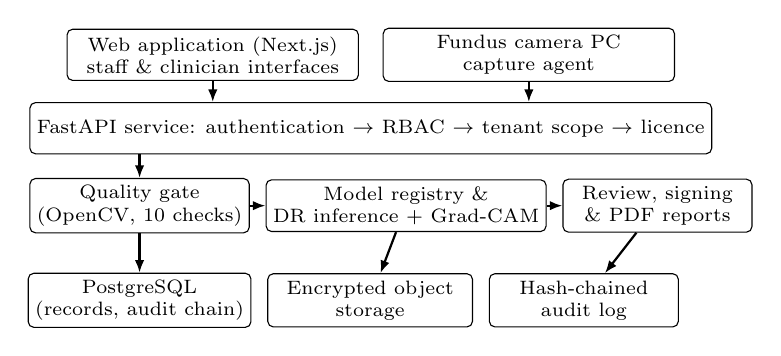
\begin{tikzpicture}[font=\scriptsize, node distance=3.5mm and 3mm,
  box/.style={draw, rounded corners=2pt, align=center, minimum height=6.5mm, inner sep=2.5pt, fill=white},
  arr/.style={-{Latex[length=1.6mm]}, thick}]
\node[box, minimum width=37mm] (web) {Web application (Next.js)\\ staff \& clinician interfaces};
\node[box, right=of web, minimum width=37mm] (cam) {Fundus camera PC\\ capture agent};
\node[box, below=6mm of $(web)!0.5!(cam)$, minimum width=78mm] (api) {FastAPI service: authentication $\rightarrow$ RBAC $\rightarrow$ tenant scope $\rightarrow$ licence};
\node[box, below=3mm of api.south west, anchor=north west, minimum width=24mm] (iqa) {Quality gate\\ (OpenCV, 10 checks)};
\node[box, right=2mm of iqa, minimum width=26mm] (ai) {Model registry \&\\ DR inference + Grad-CAM};
\node[box, right=2mm of ai, minimum width=24mm] (rep) {Review, signing\\ \& PDF reports};
\node[box, below=5mm of iqa, minimum width=24mm] (db) {PostgreSQL\\ (records, audit chain)};
\node[box, right=2mm of db, minimum width=26mm] (obj) {Encrypted object\\ storage};
\node[box, right=2mm of obj, minimum width=24mm] (aud) {Hash-chained\\ audit log};
\draw[arr] (web) -- (web|-api.north);
\draw[arr] (cam) -- (cam|-api.north);
\draw[arr] (api.south-|iqa) -- (iqa);
\draw[arr] (iqa) -- (ai);
\draw[arr] (ai) -- (rep);
\draw[arr] (iqa) -- (db);
\draw[arr] (ai) -- (obj);
\draw[arr] (rep) -- (aud);
\end{tikzpicture}
\caption{NetraRakshak architecture. Every request is authenticated, authorised by role and scoped to one hospital.}
\label{fig:arch}
\end{figure}

\subsection{Workflow}
A receptionist registers the patient and records consent separately for screening, AI analysis, data storage and
research. A technician starts a screening session and uploads right- and left-eye photographs (JPEG, PNG or TIFF). The
quality gate runs immediately. The AI step then runs on each acceptable image, after which the case enters a review
queue ordered by priority: AI-suggested referable cases first, then cases the AI could not resolve. The ophthalmologist
inspects the images in a viewer with zoom, pan, side-by-side eyes and Grad-CAM overlays, records a final grade per eye,
accepts, modifies or rejects the AI suggestion, recommends referral or recapture, and signs by re-entering their
password and attesting to the review. Only then can a report marked ``clinician approved'' be generated; earlier
reports carry a ``draft'' watermark. Signed sessions are locked.

\subsection{Multi-Tenancy and Security}
The platform serves multiple hospitals with five roles (platform administrator, hospital administrator,
ophthalmologist, screening technician, receptionist) and a role--permission matrix. Every query on patient data is
filtered by the user's hospital, and records of other hospitals return ``not found'' rather than ``forbidden''.
Platform administrators manage plans and licences but cannot read patient records. Passwords are hashed with bcrypt;
accounts lock after repeated failures; access tokens are short-lived and bound to revocable server-side sessions. An
append-only audit log records logins, views, uploads, AI runs, reviews, signatures and downloads, each entry chained
to the previous one with SHA-256 so that tampering is detectable. The model registry verifies the SHA-256 of model
weights against the model card before loading.

\subsection{Image Quality Assessment}
Table~\ref{tab:iqa} lists the checks run before any inference, on a resized copy of the image within a segmented
retinal mask. Any failure yields ``recapture required'' with a plain-language reason; three or more borderline results
yield ``inconclusive''. The thresholds are documented defaults that must be calibrated per camera against clinician
gradability labels. The checks take about 73\,ms per image.

\begin{table}[t]
\caption{Automatic Image Quality Checks}
\label{tab:iqa}
\centering\scriptsize
\begin{tabular}{@{}ll@{}}
\toprule
Check & Measurement \\
\midrule
Resolution & short side in pixels ($\geq$512 required) \\
Retinal visibility & fraction of frame covered by the retinal mask \\
Field of view & offset of the mask centroid from the image centre \\
Fundus plausibility & red-channel dominance within the mask \\
Brightness & mean luminance inside the eroded mask \\
Contrast & standard deviation of the green channel \\
Exposure & fraction of clipped and crushed pixels \\
Blur & variance of the Laplacian (CLAHE-enhanced green) \\
Focus & Tenengrad (mean squared Sobel gradient) \\
Artefacts & quadrant illumination spread, specular blobs \\
\bottomrule
\end{tabular}
\end{table}

\section{Deep Learning Method}
\subsection{Dataset}
The model was trained on the APTOS 2019 Blindness Detection dataset~\cite{aptos2019}: 3,662 colour fundus images
graded 0--4 on the International Clinical DR scale~\cite{wilkinson2003}. The data were split into training (2,615),
validation (523) and test (524) sets, stratified by grade (Table~\ref{tab:data}). APTOS does not publish patient
identifiers, so grouping was at image level. The data were used under the competition terms accepted by the account
holder; commercial use has not been confirmed.

\begin{table}[t]
\caption{Images per ICDR Grade in Each Split}
\label{tab:data}
\centering\scriptsize
\begin{tabular}{@{}lrrrrrr@{}}
\toprule
Split & No DR & Mild & Moderate & Severe & PDR & Total \\
\midrule
Train & 1281 & 281 & 710 & 134 & 209 & 2615 \\
Validation & 251 & 43 & 156 & 34 & 39 & 523 \\
Test & 273 & 46 & 133 & 25 & 47 & 524 \\
\bottomrule
\end{tabular}
\end{table}

\subsection{Preprocessing and Augmentation}
Each image is cropped to the retinal field, padded to a square, resized to $384\times384$ pixels and normalised for
illumination with Graham's local-average subtraction~\cite{graham2015},
$I' = 4I - 4\,G_\sigma * I + 128$ with $\sigma$ equal to one-thirtieth of the image size, then standardised with
ImageNet statistics. The same code path is used for training and inference. Training augmentation consists of random
horizontal and vertical flips, rotation by up to $180^\circ$, scaling by 0.92--1.10 and mild brightness and contrast
changes.

\subsection{Model and Training}
The classifier is EfficientNet-B0~\cite{tan2019} initialised with ImageNet weights~\cite{deng2009}, with its head
replaced by dropout ($p=0.3$) and a five-way linear layer (4.0\,M parameters). Class imbalance was addressed with a
class-weighted cross-entropy loss (weights inversely proportional to class frequency) with label smoothing of 0.05.
Training used AdamW (learning rate $3\times10^{-4}$, weight decay $10^{-4}$) with a one-cycle schedule, a batch size of
24 and mixed precision on a single GPU. Model selection used the validation quadratic weighted kappa~\cite{cohen1968};
training stopped after 14 epochs, and the best checkpoint was from epoch 8 (validation kappa 0.887).

\subsection{Calibration, Uncertainty and Explainability}
A temperature $T$ was fitted on the validation logits by minimising the negative log-likelihood~\cite{guo2017}, giving
$T = 0.771$. For an image with calibrated probabilities $p_k = \mathrm{softmax}(z/T)_k$, the system reports the top
class with confidence $c = \max_k p_k$ and the normalised entropy $H = -\sum_k p_k \log p_k / \log 5$. If $c < 0.60$ or
$H > 0.75$, the displayed result is ``inconclusive --- human review required''. Grad-CAM~\cite{selvaraju2017} is
computed on the final convolutional block for the predicted class and stored as an overlay and a heatmap, which are
labelled in the interface and the report as model explainability rather than lesions.

\section{Results}
\subsection{Held-Out Test Performance}
All metrics in this section were computed automatically by the training pipeline from the 524 test images, which were
not used for training, model selection or calibration (Table~\ref{tab:metrics}, Table~\ref{tab:perclass},
Fig.~\ref{fig:cm}).

\begin{table}[t]
\caption{Test-Set Performance (n = 524)}
\label{tab:metrics}
\centering\scriptsize
\begin{tabular}{@{}lr@{}}
\toprule
Metric & Value \\
\midrule
Accuracy (5-class) & 81.9\% \\
Quadratic weighted kappa & 0.876 \\
Macro precision / recall / F1 & 68.0\% / 67.8\% / 67.0\% \\
Weighted F1 & 82.1\% \\
Macro ROC-AUC (one-vs-rest) & 0.917 \\
\midrule
Referable DR sensitivity & 82.0\% (168/205) \\
Referable DR specificity & 96.6\% (308/319) \\
Referable DR PPV / NPV & 93.9\% / 89.3\% \\
Referable DR ROC-AUC & 0.981 \\
\midrule
Expected calibration error, before / after scaling & 12.2\% / 6.1\% \\
\bottomrule
\end{tabular}
\end{table}

\begin{table}[t]
\caption{Per-Class Test Performance}
\label{tab:perclass}
\centering\scriptsize
\begin{tabular}{@{}lrrrrr@{}}
\toprule
Grade & Sens. & Spec. & Prec. & F1 & AUC \\
\midrule
No apparent DR & 99.3\% & 96.8\% & 97.1\% & 0.982 & 0.998 \\
Mild NPDR & 71.7\% & 93.1\% & 50.0\% & 0.589 & 0.935 \\
Moderate NPDR & 64.7\% & 93.1\% & 76.1\% & 0.699 & 0.946 \\
Severe NPDR & 44.0\% & 95.8\% & 34.4\% & 0.386 & 0.810 \\
Proliferative DR & 59.6\% & 98.7\% & 82.4\% & 0.691 & 0.895 \\
\bottomrule
\end{tabular}
\end{table}

\begin{figure*}[t]
\centering
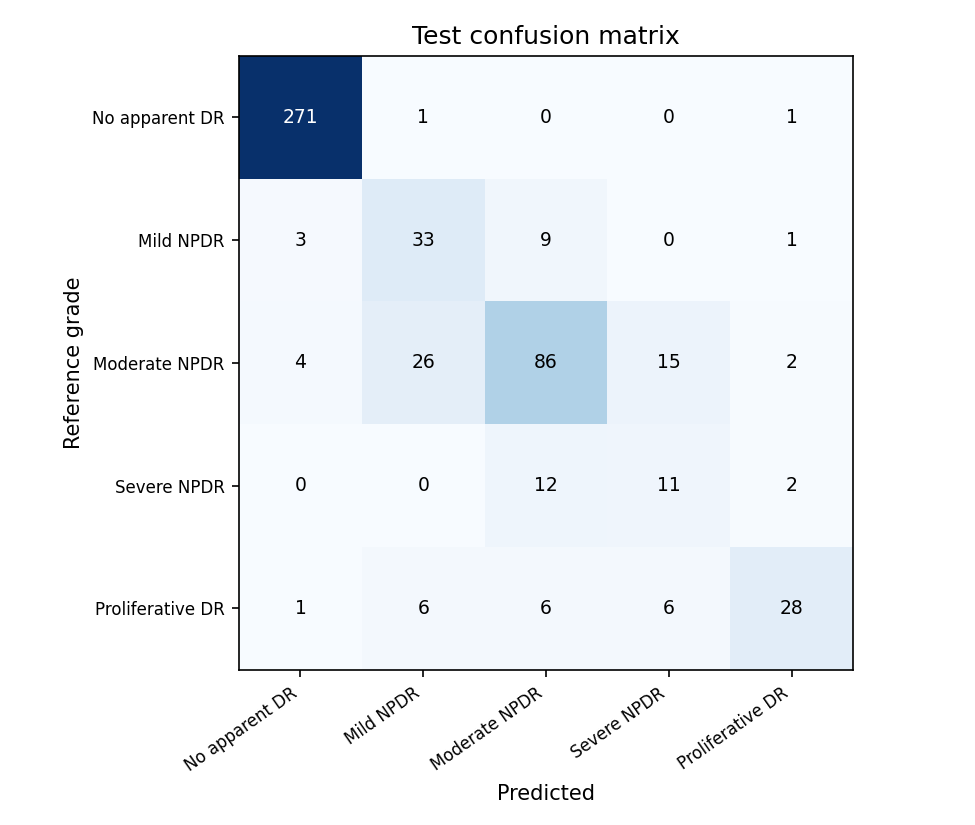
\includegraphics[height=6.2cm]{figures/confusion_matrix.png}\hspace{1.2cm}
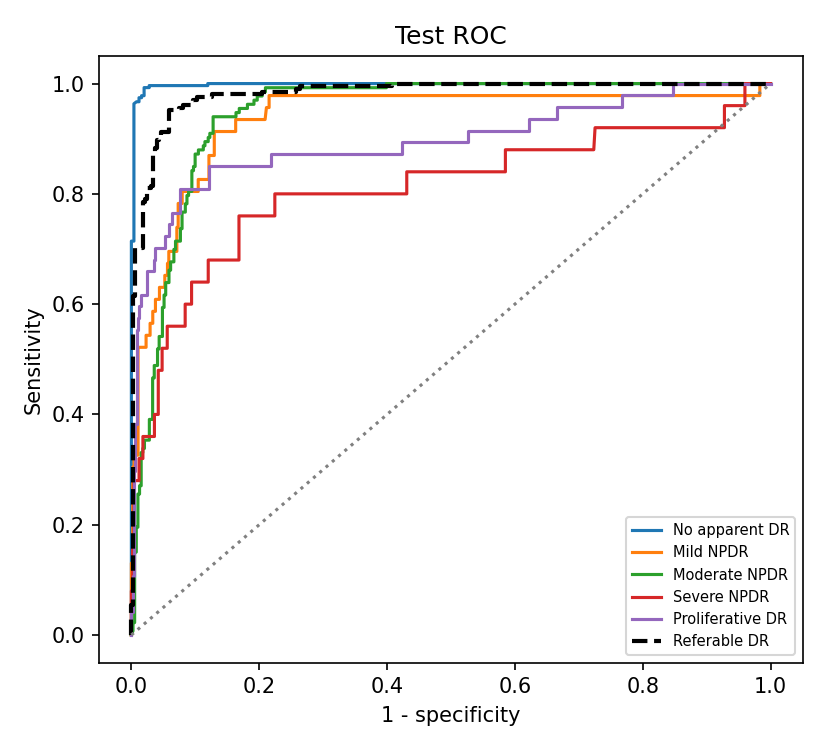
\includegraphics[height=6.2cm]{figures/roc_curves.png}
\caption{Held-out test set (n = 524): confusion matrix (left) and ROC curves per grade and for referable DR (right).}
\label{fig:cm}
\end{figure*}

\subsection{System Verification}
The backend has 30 automated tests covering authentication and lockout, role permissions, isolation between hospitals,
patient management and consent, upload validation, image quality, AI gating (model unavailable, synthetic or tampered
models, poor quality, missing consent, uncertainty), clinician signing, report status and the audit chain. All pass. A
browser-based end-to-end test reproduced the full workflow --- administrator login, registration, upload of both eyes,
quality check, AI grading with Grad-CAM, review and signature, PDF generation and dashboard update --- in production
configuration on PostgreSQL. On a two-core 2.1\,GHz CPU, inference including Grad-CAM had a median latency of 304\,ms
per eye (90th percentile 331\,ms). Fig.~\ref{fig:ui} shows the clinician review workspace.

\begin{figure}[t]
\centering
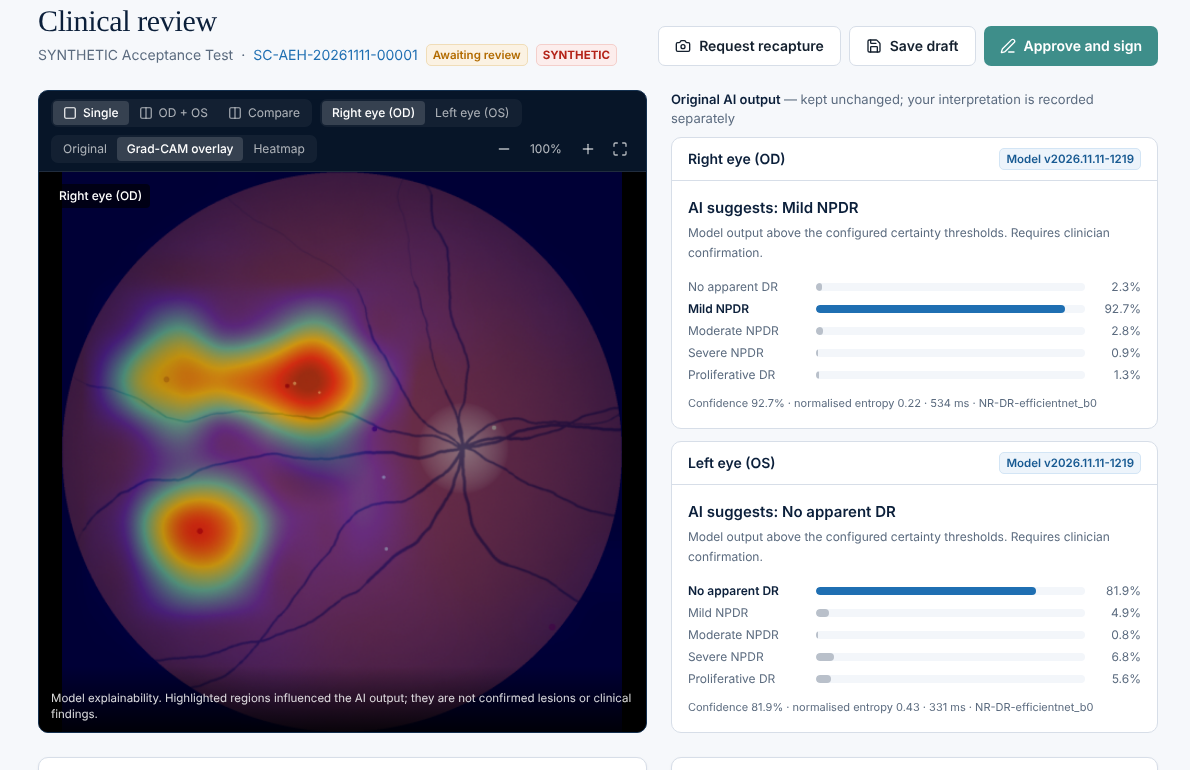
\includegraphics[width=\columnwidth]{figures/ui_review.png}
\caption{Clinician review workspace with a synthetic test patient: Grad-CAM overlay, the unmodified AI output with
calibrated probabilities, and per-eye accept, modify or reject decisions.}
\label{fig:ui}
\end{figure}

\section{Discussion}
\subsection{Clinical Interpretation}
The model distinguishes eyes without DR well (sensitivity 99.3\%) and has high specificity for referable disease, but
at the default operating point it graded 37 of 205 referable eyes (18\%) as non-referable, mostly moderate NPDR graded
as mild (Fig.~\ref{fig:cm}). Severe NPDR, with only 25 test images, is the weakest class. These results justify the
design choice that every case is reviewed and signed by an ophthalmologist; the model must not be used to rule out
disease. Tuning the uncertainty thresholds on validation data could route more moderate-versus-mild ambiguity to the
``inconclusive'' path.

\subsection{Limitations}
First, APTOS lacks patient identifiers, so both eyes of one person may fall into different splits, which can make the
results optimistic. Second, the data come from a single source, and performance on other cameras, populations and
dilation protocols is unknown; no external validation (for example on IDRiD~\cite{porwal2018}) has been performed.
Third, the quality gate checks image properties, not whether the content is a gradable retina: in testing, the model
gave confident outputs on procedurally generated synthetic images, so an out-of-distribution detector is needed.
Fourth, the model does not assess diabetic macular oedema. Fifth, clinical validation has not been carried out.

\subsection{Regulatory and Ethical Considerations}
Software intended for screening or diagnosis is a medical device under India's Medical Devices Rules, 2017. CDSCO's
draft guidance on medical device software (October 2025) classifies software by the significance of its output and
the seriousness of the condition, requires lifecycle quality management, risk management and clinical evaluation, and
introduces an algorithm change protocol for AI model updates~\cite{cdsco2025}. The project includes draft
intended-use, risk-management (ISO~14971~\cite{iso14971}), software-requirements, cybersecurity and validation-plan
documents and is structured for IEC~62304~\cite{iec62304}. Patient data handling follows the purpose-specific consent
and erasure model of the Digital Personal Data Protection Act, 2023~\cite{dpdp2023}. The platform has not been
classified, licensed or certified.

\section{Conclusion and Future Work}
NetraRakshak shows that an AI grading model can be embedded in a complete, auditable, clinician-supervised screening
workflow with quality control, calibrated uncertainty and explainability. The DR model reached a referable-DR
sensitivity of 82.0\% and specificity of 96.6\% on held-out APTOS data. Future work comprises training on licensed,
patient-grouped Indian data from several camera types; external validation; an out-of-distribution detector;
diabetic macular oedema assessment; tuning the uncertainty operating point; a prospective multi-centre clinical
validation study with ethics approval; and a CDSCO submission. Further disease modules will be activated only after
their own training and validation.

\section*{Acknowledgment}
The APTOS 2019 data were provided by the Asia Pacific Tele-Ophthalmology Society through Kaggle. All patient records and
images shown in this report are synthetic.

\begin{thebibliography}{99}
\bibitem{gulshan2016} V.~Gulshan \textit{et al.}, ``Development and validation of a deep learning algorithm for
detection of diabetic retinopathy in retinal fundus photographs,'' \textit{JAMA}, vol.~316, no.~22, pp.~2402--2410, 2016.
\bibitem{ting2017} D.~S.~W.~Ting \textit{et al.}, ``Development and validation of a deep learning system for diabetic
retinopathy and related eye diseases using retinal images from multiethnic populations with diabetes,''
\textit{JAMA}, vol.~318, no.~22, pp.~2211--2223, 2017.
\bibitem{abramoff2018} M.~D.~Abr\`amoff, P.~T.~Lavin, M.~Birch, N.~Shah, and J.~C.~Folk, ``Pivotal trial of an
autonomous AI-based diagnostic system for detection of diabetic retinopathy in primary care offices,''
\textit{npj Digit. Med.}, vol.~1, art.~39, 2018.
\bibitem{ruamviboonsuk2019} P.~Ruamviboonsuk \textit{et al.}, ``Deep learning versus human graders for classifying
diabetic retinopathy severity in a nationwide screening program,'' \textit{npj Digit. Med.}, vol.~2, art.~25, 2019.
\bibitem{rajalakshmi2018} R.~Rajalakshmi \textit{et al.}, ``Automated diabetic retinopathy detection in smartphone-based
fundus photography using artificial intelligence,'' \textit{Eye}, vol.~32, pp.~1138--1144, 2018.
\bibitem{aptos2019} Asia Pacific Tele-Ophthalmology Society, ``APTOS 2019 Blindness Detection,'' Kaggle, 2019.
[Online]. Available: \url{https://www.kaggle.com/competitions/aptos2019-blindness-detection}
\bibitem{porwal2018} P.~Porwal \textit{et al.}, ``Indian Diabetic Retinopathy Image Dataset (IDRiD): A database for
diabetic retinopathy screening research,'' \textit{Data}, vol.~3, no.~3, art.~25, 2018.
\bibitem{wilkinson2003} C.~P.~Wilkinson \textit{et al.}, ``Proposed international clinical diabetic retinopathy and
diabetic macular edema disease severity scales,'' \textit{Ophthalmology}, vol.~110, no.~9, pp.~1677--1682, 2003.
\bibitem{graham2015} B.~Graham, ``Kaggle diabetic retinopathy detection competition report,'' Univ. of Warwick, 2015.
\bibitem{tan2019} M.~Tan and Q.~V.~Le, ``EfficientNet: Rethinking model scaling for convolutional neural networks,''
in \textit{Proc. 36th Int. Conf. Mach. Learn. (ICML)}, 2019, pp.~6105--6114.
\bibitem{deng2009} J.~Deng, W.~Dong, R.~Socher, L.-J.~Li, K.~Li, and L.~Fei-Fei, ``ImageNet: A large-scale
hierarchical image database,'' in \textit{Proc. IEEE Conf. Comput. Vis. Pattern Recognit. (CVPR)}, 2009, pp.~248--255.
\bibitem{cohen1968} J.~Cohen, ``Weighted kappa: Nominal scale agreement with provision for scaled disagreement or
partial credit,'' \textit{Psychol. Bull.}, vol.~70, no.~4, pp.~213--220, 1968.
\bibitem{guo2017} C.~Guo, G.~Pleiss, Y.~Sun, and K.~Q.~Weinberger, ``On calibration of modern neural networks,'' in
\textit{Proc. 34th Int. Conf. Mach. Learn. (ICML)}, 2017, pp.~1321--1330.
\bibitem{selvaraju2017} R.~R.~Selvaraju, M.~Cogswell, A.~Das, R.~Vedantam, D.~Parikh, and D.~Batra, ``Grad-CAM: Visual
explanations from deep networks via gradient-based localization,'' in \textit{Proc. IEEE Int. Conf. Comput. Vis.
(ICCV)}, 2017, pp.~618--626.
\bibitem{cdsco2025} Central Drugs Standard Control Organisation, ``Draft guidance document on medical device
software,'' Ministry of Health and Family Welfare, Govt. of India, Oct. 2025.
\bibitem{iso14971} \textit{Medical Devices --- Application of Risk Management to Medical Devices}, ISO 14971:2019.
\bibitem{iec62304} \textit{Medical Device Software --- Software Life Cycle Processes}, IEC 62304:2006+A1:2015.
\bibitem{dpdp2023} \textit{The Digital Personal Data Protection Act, 2023}, Act No.~22 of 2023, Govt. of India.
\end{thebibliography}

\end{document}
